% Sección: La identidad de Euler
\section{La identidad de Euler: $e^{i\pi} = -1$}\label{sec:geom}

La identidad de Euler es una de las fórmulas más elegantes de las matemáticas, conectando cinco constantes fundamentales: $e$, $i$, $\pi$, $1$ y $0$.

\begin{theorem}[Identidad de Euler]
$$e^{i\pi} + 1 = 0$$
o equivalentemente:
$$e^{i\pi} = -1$$
\end{theorem}

\subsection{Demostración usando la fórmula de Euler}

La fórmula de Euler establece que para cualquier número real $\theta$:
\begin{equation}\label{eq:euler_formula}
e^{i\theta} = \cos(\theta) + i\sin(\theta)
\end{equation}

Esta fórmula se puede demostrar usando las series de Taylor:
\begin{align}
e^x &= \sum_{n=0}^{\infty} \frac{x^n}{n!} = 1 + x + \frac{x^2}{2!} + \frac{x^3}{3!} + \frac{x^4}{4!} + \cdots \\
\cos(x) &= \sum_{n=0}^{\infty} \frac{(-1)^n x^{2n}}{(2n)!} = 1 - \frac{x^2}{2!} + \frac{x^4}{4!} - \frac{x^6}{6!} + \cdots \\
\sin(x) &= \sum_{n=0}^{\infty} \frac{(-1)^n x^{2n+1}}{(2n+1)!} = x - \frac{x^3}{3!} + \frac{x^5}{5!} - \frac{x^7}{7!} + \cdots
\end{align}

Sustituyendo $x = i\theta$ en la serie de $e^x$:
\begin{align}
e^{i\theta} &= 1 + i\theta + \frac{(i\theta)^2}{2!} + \frac{(i\theta)^3}{3!} + \frac{(i\theta)^4}{4!} + \cdots \\
&= 1 + i\theta - \frac{\theta^2}{2!} - i\frac{\theta^3}{3!} + \frac{\theta^4}{4!} + \cdots
\end{align}

Separando las partes real e imaginaria:
\begin{align}
e^{i\theta} &= \left(1 - \frac{\theta^2}{2!} + \frac{\theta^4}{4!} - \cdots\right) + i\left(\theta - \frac{\theta^3}{3!} + \frac{\theta^5}{5!} - \cdots\right) \\
&= \cos(\theta) + i\sin(\theta)
\end{align}

\subsection{Aplicación para $\theta = \pi$}

Ahora, aplicando la fórmula de Euler con $\theta = \pi$:
\begin{equation}
e^{i\pi} = \cos(\pi) + i\sin(\pi)
\end{equation}

Sabemos que:
\begin{itemize}
\item $\cos(\pi) = -1$
\item $\sin(\pi) = 0$
\end{itemize}

Por lo tanto:
\begin{equation}
e^{i\pi} = -1 + i \cdot 0 = -1
\end{equation}

\subsection{Interpretación geométrica}

En el plano complejo, $e^{i\theta}$ representa un punto en el círculo unitario en el ángulo $\theta$ desde el eje real positivo. Cuando $\theta = \pi$, estamos en el punto diametralmente opuesto al punto $(1,0)$, que es exactamente $(-1,0)$, confirmando que $e^{i\pi} = -1$.

\begin{center}
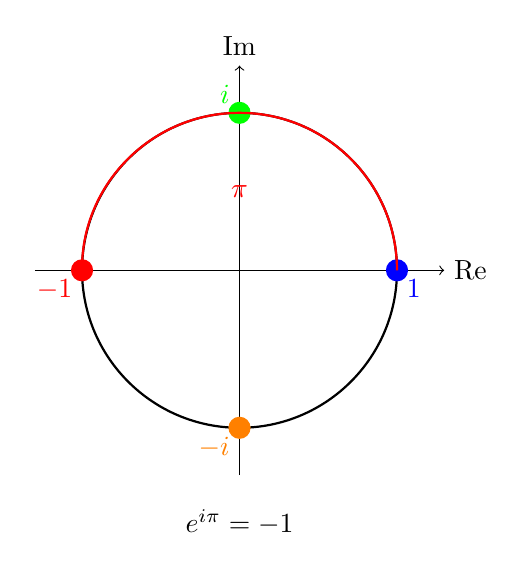
\begin{tikzpicture}[scale=2]
  % Círculo unitario
  \draw[thick] (0,0) circle(1);
  
  % Ejes
  \draw[->] (-1.3,0) -- (1.3,0) node[right] {Re};
  \draw[->] (0,-1.3) -- (0,1.3) node[above] {Im};
  
  % Puntos importantes
  \fill[blue] (1,0) circle (2pt) node[below right] {$1$};
  \fill[red] (-1,0) circle (2pt) node[below left] {$-1$};
  \fill[green] (0,1) circle (2pt) node[above left] {$i$};
  \fill[orange] (0,-1) circle (2pt) node[below left] {$-i$};
  
  % Arco para mostrar π
  \draw[thick, red, ->] (1,0) arc (0:180:1);
  \node[red] at (0,0.5) {$\pi$};
  
  % Etiquetas
  \node at (0,-1.6) {$e^{i\pi} = -1$};
\end{tikzpicture}
\end{center}
